\section{ShopChain}
Il sito di ShopChain presenta uno schema a tre pannelli che verrà mantenuto in ogni pagina interna allo stesso.\\
La figura seguente evidenzia in maniera specifica i tre pannelli usando i colori
\begin{itemize}
    \item \textbf{Giallo}: navbar
    \item \textbf{Verde}: menu di navigazione
    \item \textbf{Rosso}: contenuto
\end{itemize}
\begin{figure}[H]
    \centering
    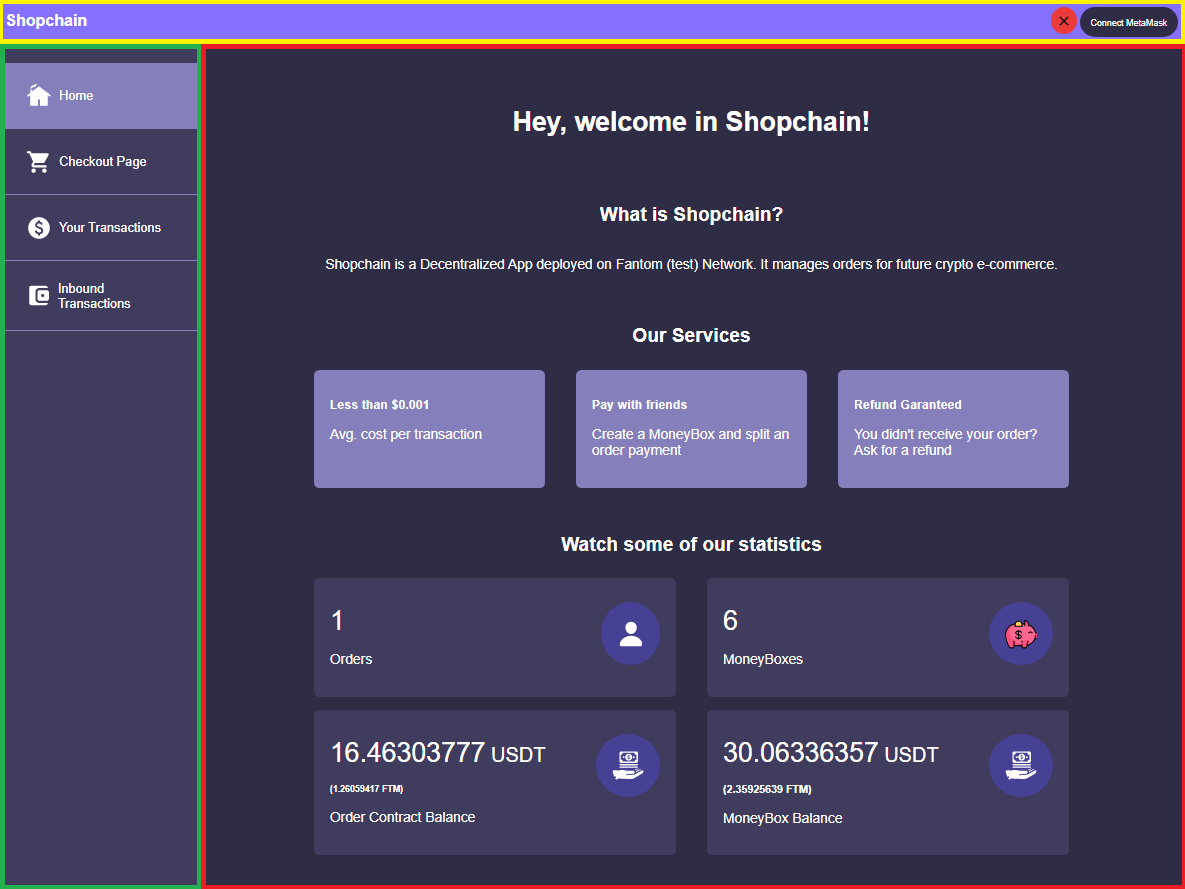
\includegraphics[scale=0.2]{immagini/trePannelli.png}
    \caption{Schema a tre pannelli}
\end{figure}


    \subsection{Navbar}
    La navbar presenta la scritta Shopchain cliccabile che rimanda direttamente alla home, lo stato della connessione a MetaMask e l'indirizzo del portafoglio connesso.
    \begin{figure}[H]
        \centering
        
\includegraphics[scale=0.5]{immagini/navbar.png}
        \caption{navbar}
    \end{figure}
    \textbf{}\\
    La prima cosa da fare una volta all'interno del sito è effettuare quindi la connessione a MetaMask. Per farlo e sufficiente cliccare il bottone "Connect MetaMask". A questo punto si aprirà un popup dell'estensione che chiederà di inserire la password scelta al momento dell'iscrizione. Una volta inserita la Password la connessione sarà stabilita.\\
    L'icona alla sinistra dell'indirizzo del portafoglio segnala appunto lo stato della connessione alla rete Fantom\glo{}.\\
    Posizionandosi sopra l'icona sarà possibile reperire eventuali messaggi di errore:
    \begin{figure}[H]
        \centering
        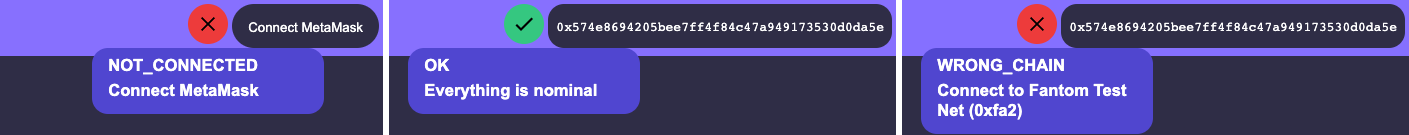
\includegraphics[scale=0.4]{immagini/stateSignal.png}
        \caption{messaggi di stato}
    \end{figure}

    \subsection{Menù e Contenuto}
    Il menù di navigazione presenta le seguenti sezioni:
    \begin{itemize}
        \item \textbf{Home};
        \item \textbf{Checkout Page};
        \item \textbf{Your Transactions};
        \item \textbf{Inbound Transactions};
    \end{itemize}

    Tutte le sezioni sopracitate vengono poi visualizzate all'interno del pannello dei contenuti.

    
        \subsubsection{Home}
        La home di ShopChain contiene solamente alcune informazioni riguardanti il sito stesso.
        \begin{figure}[H]
            \centering
            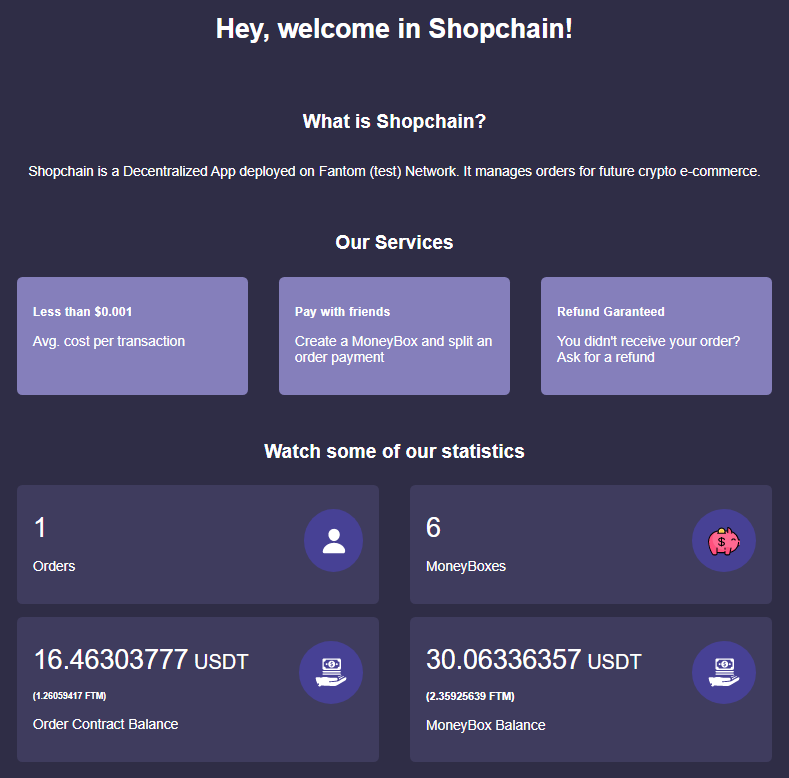
\includegraphics[scale=0.2]{immagini/Home.png}
            \caption{HomePage di ShopChain}
        \end{figure}
        \textbf{}\\
        Potrebbe risultare interessante dare uno sguardo alle statistiche riguardanti il contratto:
        \begin{figure}[H]
            \centering
            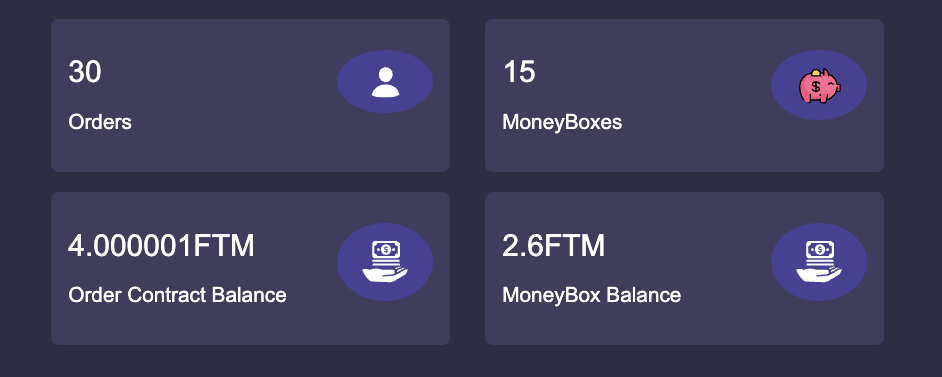
\includegraphics[scale=0.4]{immagini/ContractDetails.png}
            \caption{Statistiche contratto}
        \end{figure}
        \textbf{}\\
        Esse rappresentano gli ordini effettuati su shopchain da quando è in funzione e quanto denaro è attualmente bloccato all'interno del contratto rispettivamente per ordine singolo per le icone di sinistra e per MoneyBox le icone di destra.
        \subsubsection{Checkout Page}
        Cliccando il link alla Checkout Page nel menù verremo reindirizzati alla seguente pagina:
        \begin{figure}[H]
            \centering
            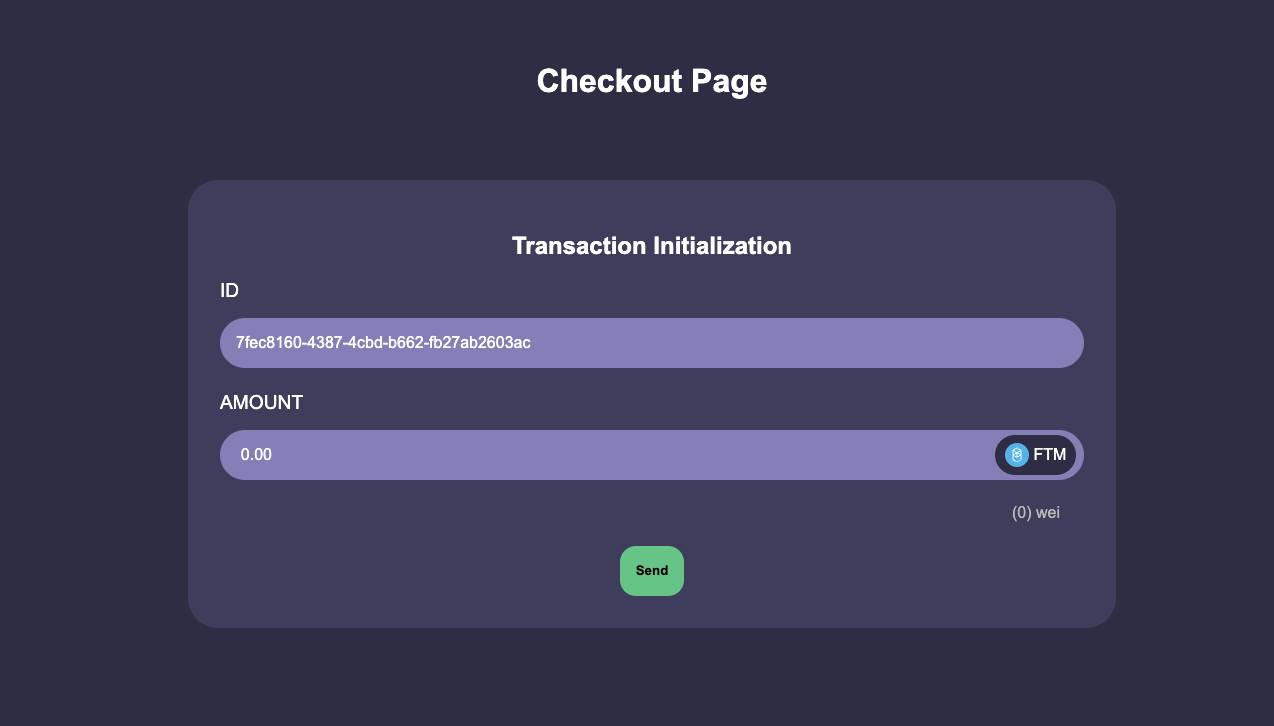
\includegraphics[scale=0.2]{immagini/Checkout/Checkout.png}
            \caption{Checkout Page}
        \end{figure}
        \textbf{}\\
        La pagina di Checkout presenta un form con i campi ID e AMOUNT.\\
        Questa pagina risulta essere esclusivamente dimostrativa in quanto tali dati saranno successivamente reperiti direttamente dall'e-commerce\glo{} e saranno impossibili da cambiare.\\
        Al momento, allo scopo di mostrare il funzionamento dell'applicativo, in quanto il sito non risulta effettivamente collegato a nessun e-commerce\glo{}, è possibile scegliere un ammontare da pagare. \\
        Una volta scelto l'importo sarà sufficiente cliccare il tasto \texttt{"Send"} per proseguire.\\\\
        A questo punto ci troveremo davanti alla pagina di scelta della modalità del pagamento:
        \begin{figure}[H]
            \centering
            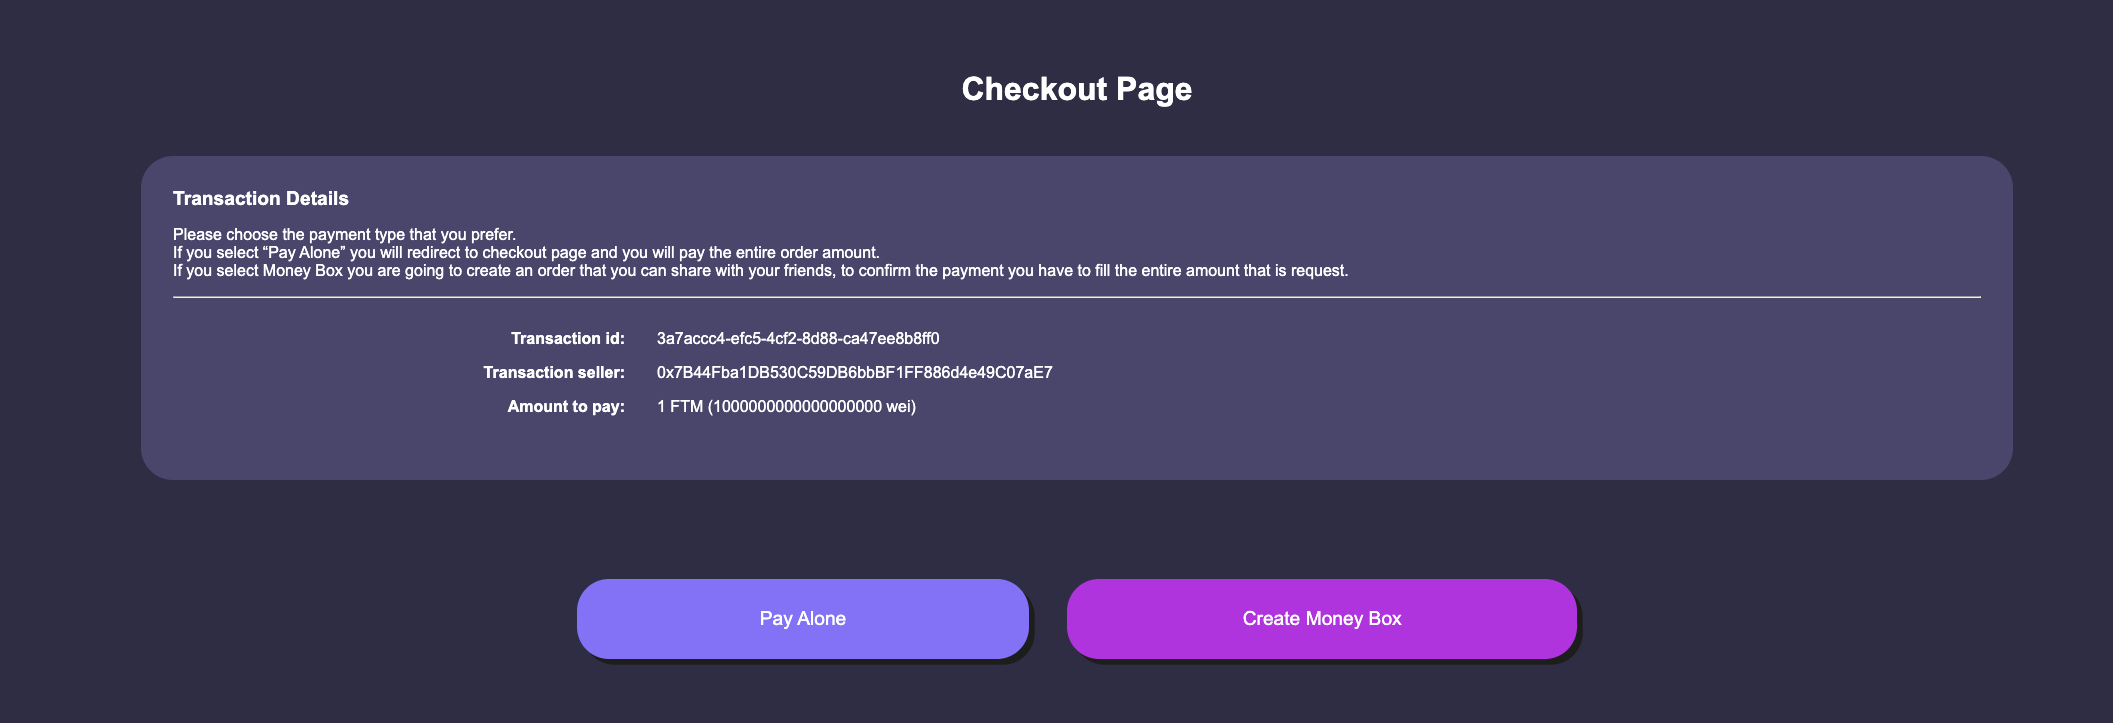
\includegraphics[scale=0.2]{immagini/Checkout/PaymentMode.png}
            \caption{Pagina di scelta modalità di pagamento}
        \end{figure}
        \textbf{}\\
        Nel particolare in questa pagina è possibile trovare il riassunto della transazione con i rispettivi indirizzi di uscita e di entrata e l'importo dell'ammontare totale della somma di pagamento.\\\\
        Nel seguito analizzeremo le differenze e i dettagli delle due modalità di pagamento.
            \paragraph{Pagamento Singolo}
            \begin{figure}[H]
                \centering
                
\includegraphics[scale=0.3]{immagini/Checkout/PayAlone.png}
                \caption{Tasto scelta modalità pagamento singolo}
            \end{figure}
            Cliccando il tasto \texttt{"Pay Alone"} verrà aperto un popup dall'estensione MetaMask con i dettagli del pagamento e la possibilità di confermare o annullare il pagamento. Un layer di caricamento apparirà nella pagina ShopChain fintantoché la transazione non sarà conclusa come mostrato nella figura seguente:
            \begin{figure}[H]
                \centering
                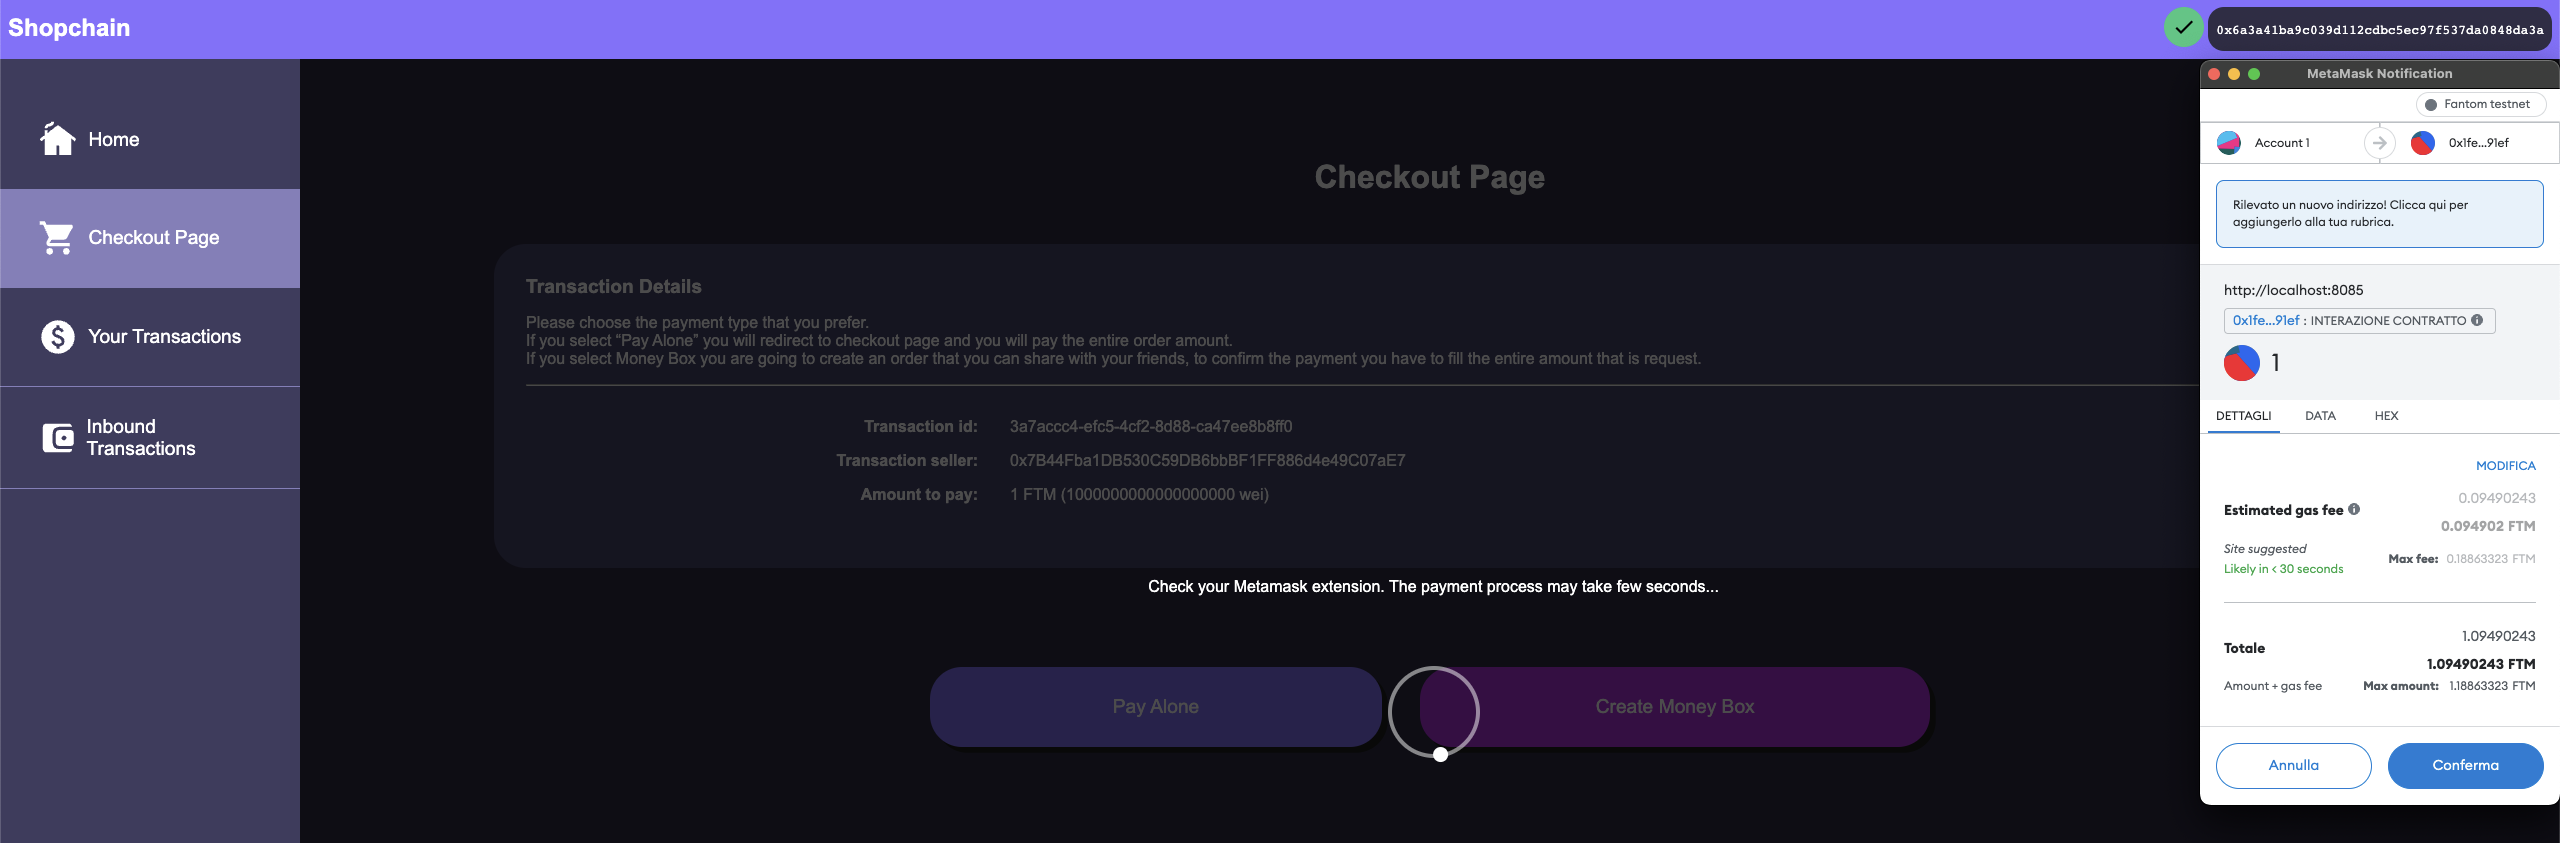
\includegraphics[scale=0.2]{immagini/Checkout/SinglePaymentLayer.png}
                \caption{Fase di pagamento singolo}
            \end{figure}
            \textbf{}\\
            Una volta che la transazione sarà stata registrata (in genere pochi secondi dopo averla confermata), si verrà reindirizzati ad una pagina che conferma che la transazione è avvenuta correttamente:
            \begin{figure}[H]
                \centering
                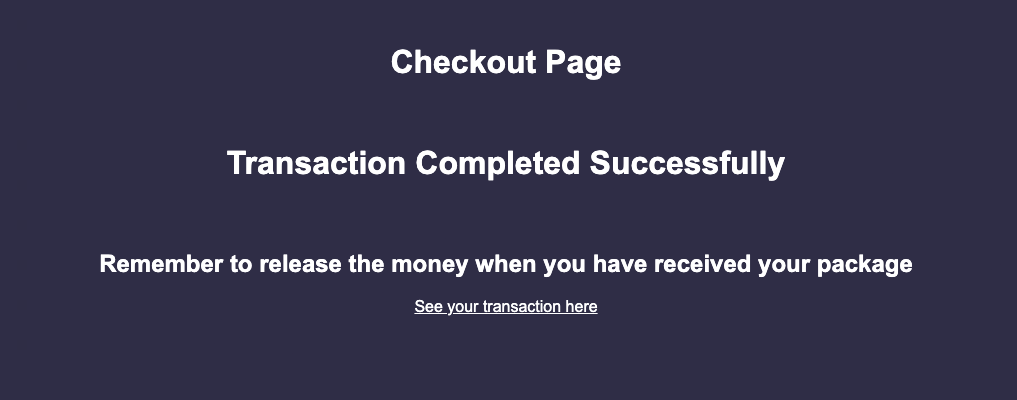
\includegraphics[scale=0.3]{immagini/Checkout/PayAloneTransactionSuccess.png}
                \caption{Transazione avvenuta con successo}
            \end{figure}
            \textbf{}\\
            Da qui sarà possibile visualizzare il dettaglio della transazione semplicemente cliccando il link \texttt{"See your transaction here"} attraverso il quale si verrà reindirizzati alla pagina mostrata di seguito:
            \begin{figure}[H]
                \centering
                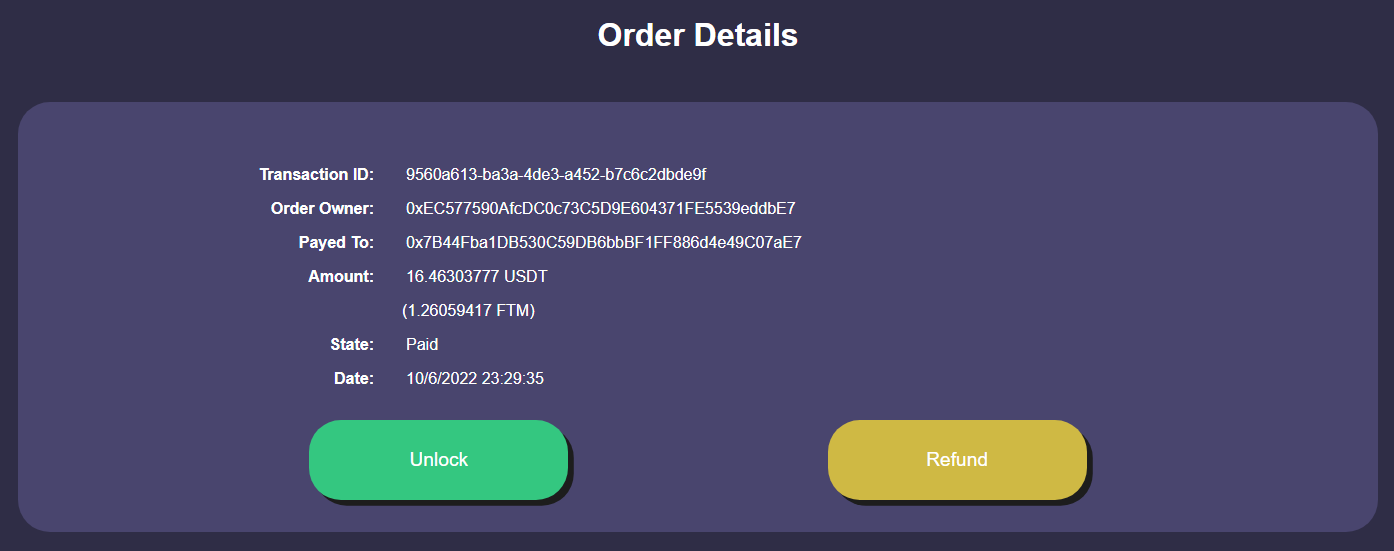
\includegraphics[scale=0.2]{immagini/Checkout/SinglePaymentDetails.png}
                \caption{Dettaglio transazione singola}
            \end{figure}
            \textbf{}\\
            Da qui sarà quindi possibile sbloccare il denaro attraverso un codice di sblocco (una volta ricevuto l'ordine) o chiedere il rimborso (qualora l'ordine non venga mai recapitato) mediante gli appositi bottoni.
            \paragraph{Pagamento MoneyBox}
            \begin{figure}[H]
                \centering
                
\includegraphics[scale=0.3]{immagini/Checkout/CreateMoneyBox.png}
                \caption{Tasto scelta modalità pagamento MoneyBox}
            \end{figure}
            Cliccando il tasto \texttt{"Create Moneybox"} verrà scelta la modalità di pagamento MoneyBox e la pagina mostrata sarà la seguente:
            \begin{figure}[H]
                \centering
                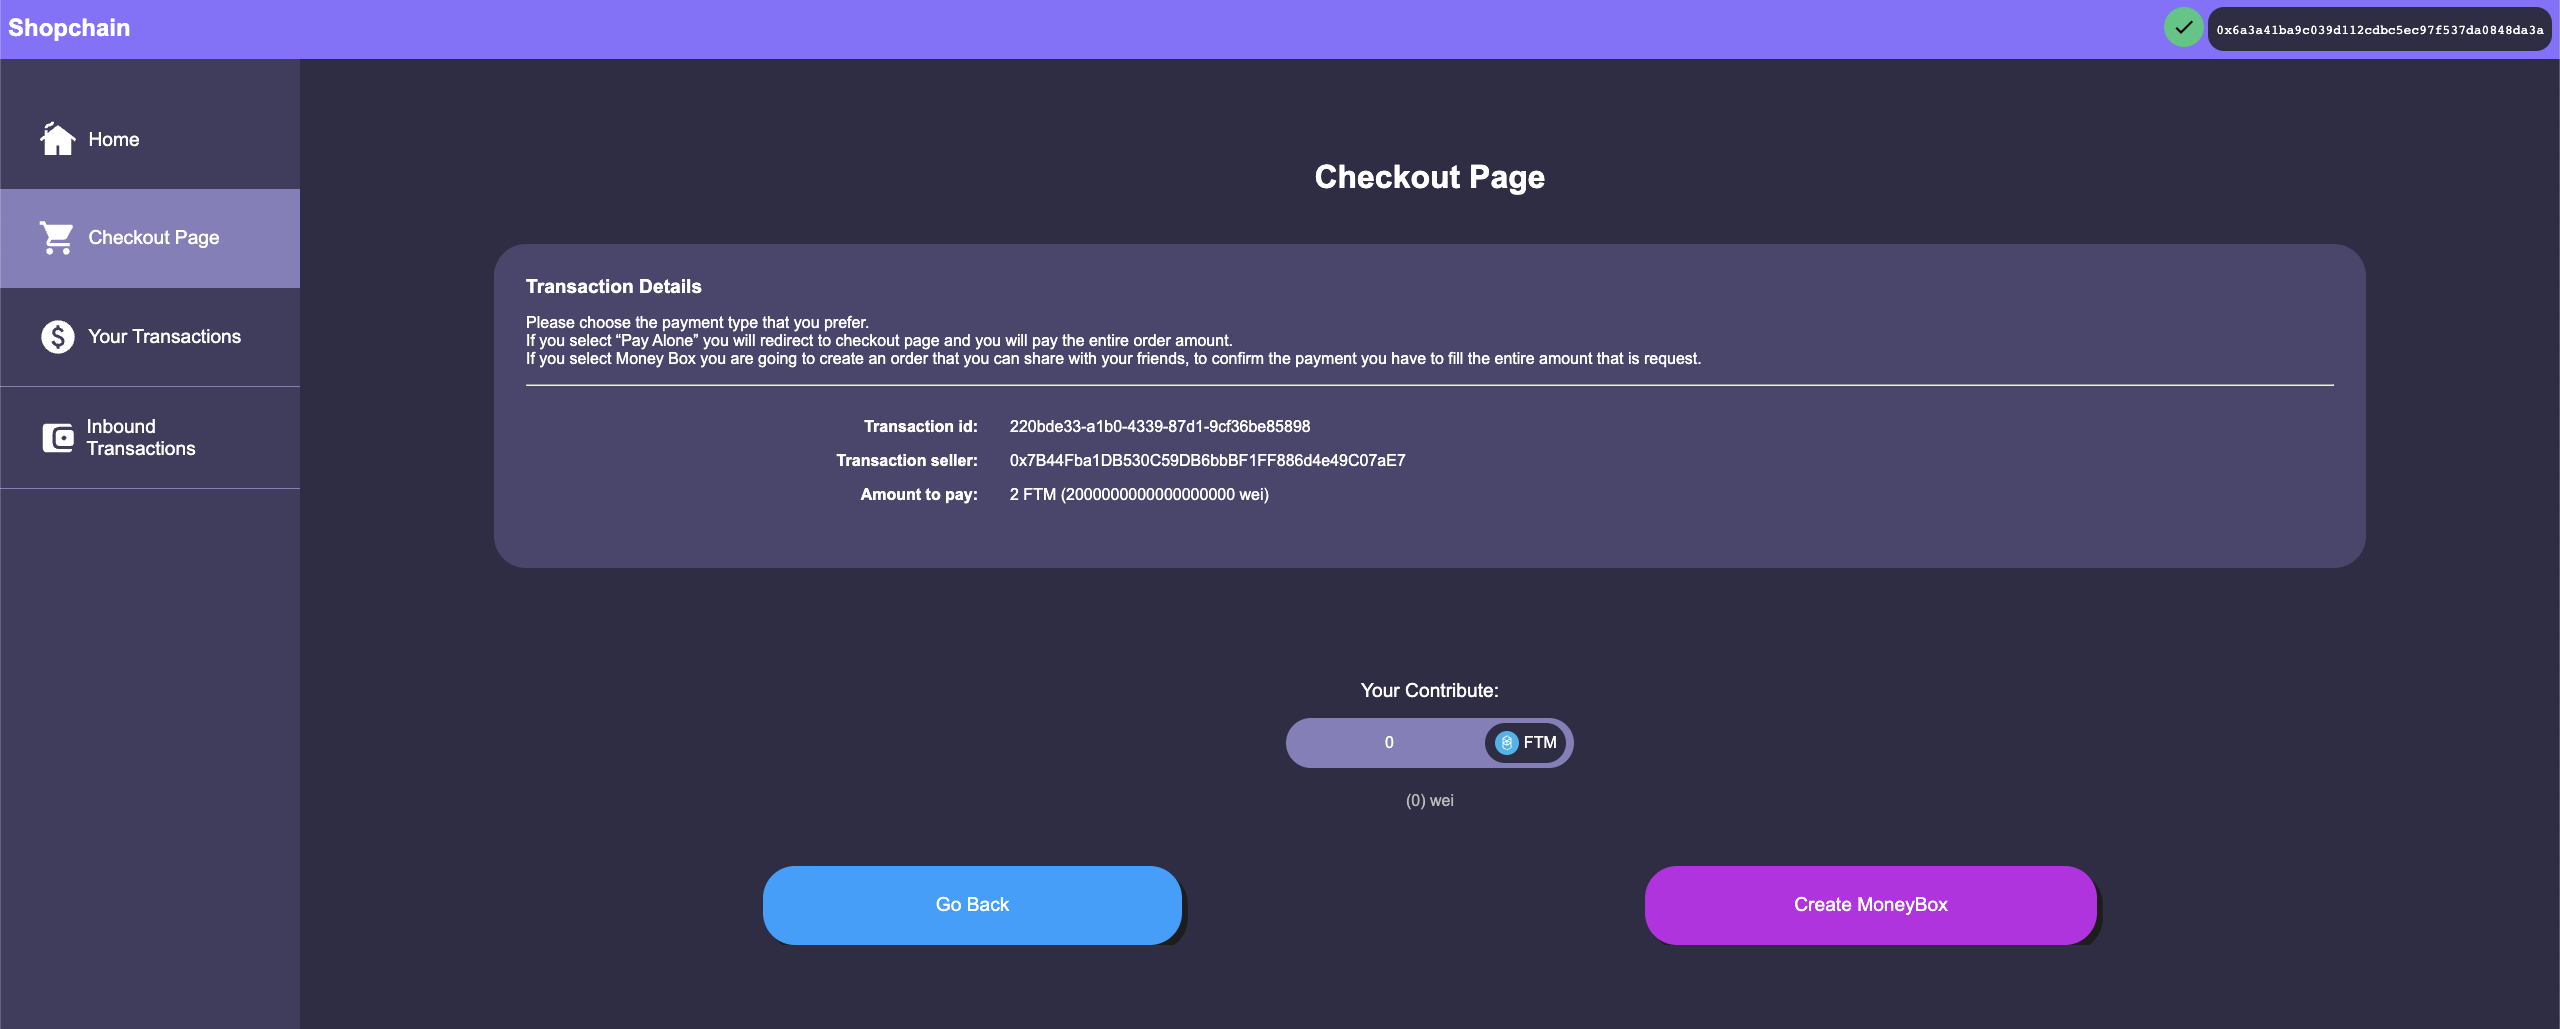
\includegraphics[scale=0.2]{immagini/Checkout/MoneyBoxCheckout.png}
                \caption{Pagina Checkout MoneyBox}
            \end{figure}
            \textbf{}\\
            Analizzando la pagina è possibile vedere il dettaglio della transazione, un box per inserire l'eventuale proprio contributo fin dalla creazione e i tasti \texttt{"Go Back"} e \texttt{"Create MoneyBox"}.\\\\
            Per inserire un contributo sarà necessario inserire l'importo all'interno del box come mostrato di seguito:
            \begin{figure}[H]
                \centering
                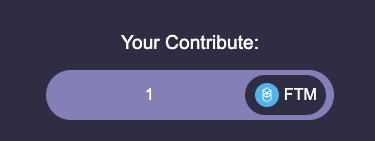
\includegraphics[scale=0.4]{immagini/Checkout/InitialContribute.png}
                \caption{Contributo MoneyBox in fase di creazione}
            \end{figure}
            \textbf{}\\
            ed in seguito cliccare il bottone \texttt{"Create MoneyBox"}.\\
            A questo punto verrà aperto un popup dall'estensione MetaMask con i dettagli del pagamento e la possibilità di confermare o annullare il pagamento. Un layer di caricamento apparirà nella pagina ShopChain fintantoché la transazione non sarà conclusa come mostrato nella figura seguente:
            \begin{figure}[H]
                \centering
                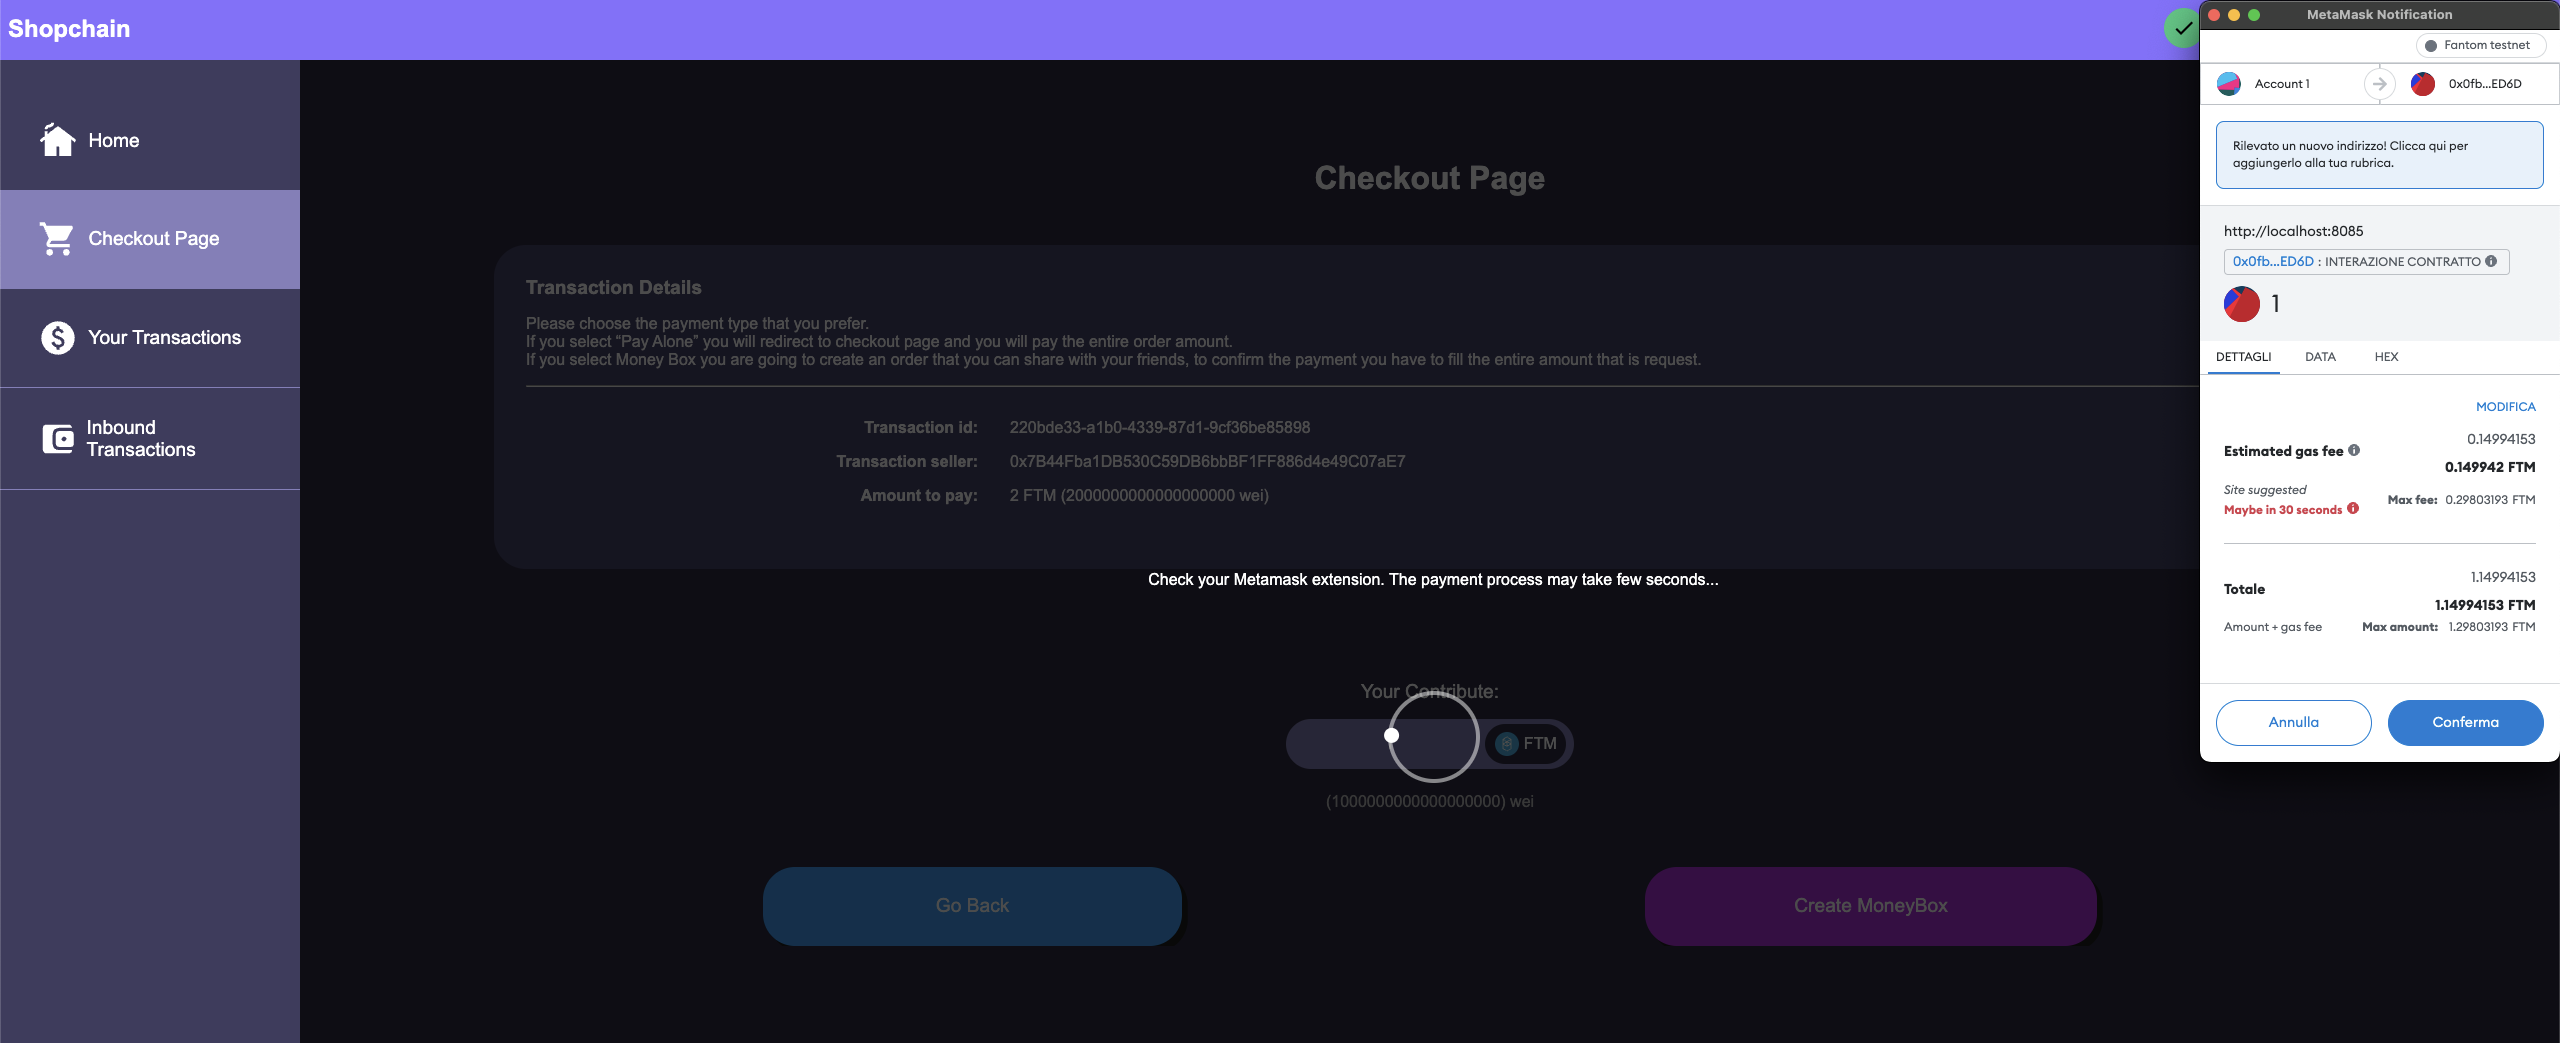
\includegraphics[scale=0.2]{immagini/Checkout/MoneyBoxLayer.png}
                \caption{Fase di pagamento MoneyBox}
            \end{figure}
            \textbf{}\\
            Una volta che la transazione sarà stata registrata (in genere pochi secondi dopo averla confermata), si verrà reindirizzati ad una pagina che conferma che la transazione è avvenuta correttamente:
            \begin{figure}[H]
                \centering
                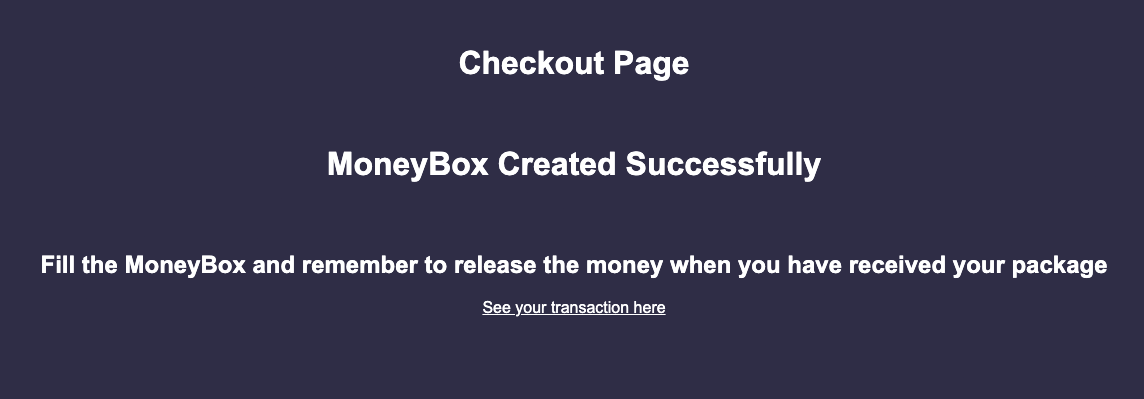
\includegraphics[scale=0.3]{immagini/Checkout/MoneyBoxTransactionSuccess.png}
                \caption{creazione Moneybox avvenuta con successo}
            \end{figure}
            \textbf{}\\
            Da qui sarà possibile visualizzare il dettaglio della transazione semplicemente cliccando il link \texttt{"See your transaction here"} attraverso il quale si verrà reindirizzati alla pagina mostrata di seguito:
            \begin{figure}[H]
                \centering
                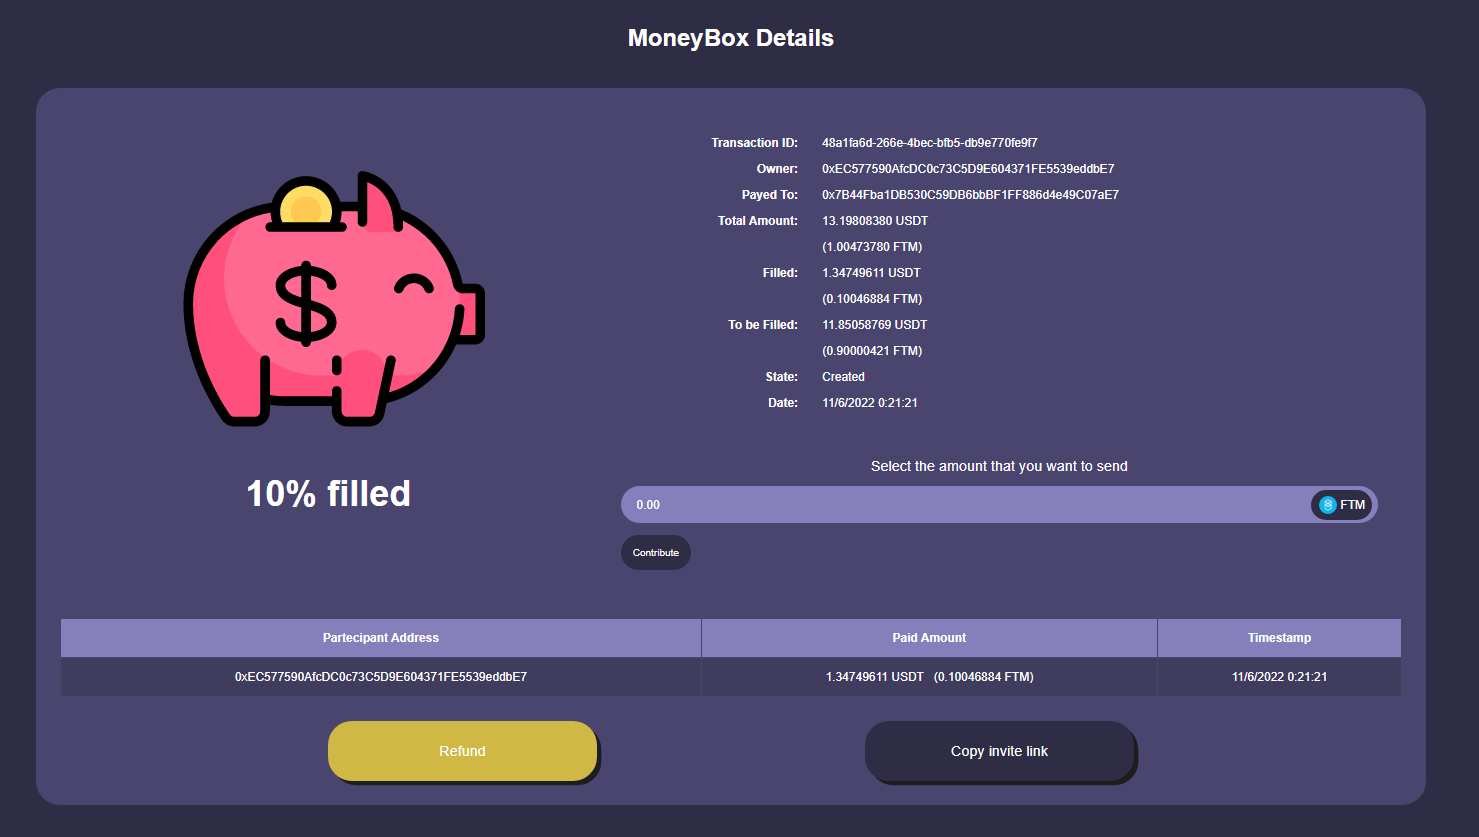
\includegraphics[scale=0.2]{immagini/Checkout/MoneyBoxDetails.png}
                \caption{Dettaglio transazione MoneyBox}
            \end{figure}
            \textbf{}\\
            Da qui sarà quindi possibile copiare il link di invito cliccando il bottone \texttt{"Copy invite link"}, da condividere con i contribuenti alla moneybox, o chiedere il rimborso qualora la moneybox debba essere annullata o l'ordine non venga mai recapitato.\\
            All'interno della pagina è inoltre possibile notare altre informazioni quali la percentuale di rempimento della moneybox, un box per contribuire alla moneybox e una tabella con il dettaglio delle transazioni dei contribuenti.\\
            Per condividere la moneybox con gli altri contribuenti sarà sufficiente condividere il link di invito precedentemente descritto e che l'utente contribuente disponga di tutti i requisiti citati fino a questo punto.\\
            Quando la MoneyBox sarà completamente riempita il suo stato passerà da \texttt{"Created"} a \texttt{"Paid"} e comparirà l'apposito bottone che permetterà di effettuare lo sblocco del denaro al wallet del venditore.\\\\ 
            \textbf{N.B.} \textit{Solo l'utente che ha creato la moneybox potrà effettuare lo sblocco.}\\\\
            Le immagini a seguire mostrano in dettaglio il box per inserire il proprio contributo, la tabella dei contribuenti e un'esempio di come la pagina si trasforma quando la moneybox passa allo stato \texttt{"Paid"}:
            \begin{figure}[H]
                \centering
                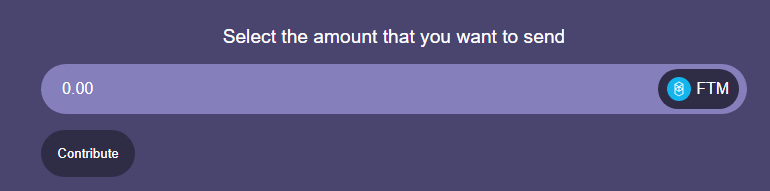
\includegraphics[scale=0.3]{immagini/Checkout/Contribute.png} 
                \caption{Box per inserire il proprio contributo alla MoneyBox}
            \end{figure}
            \begin{figure}[H]
                \centering
                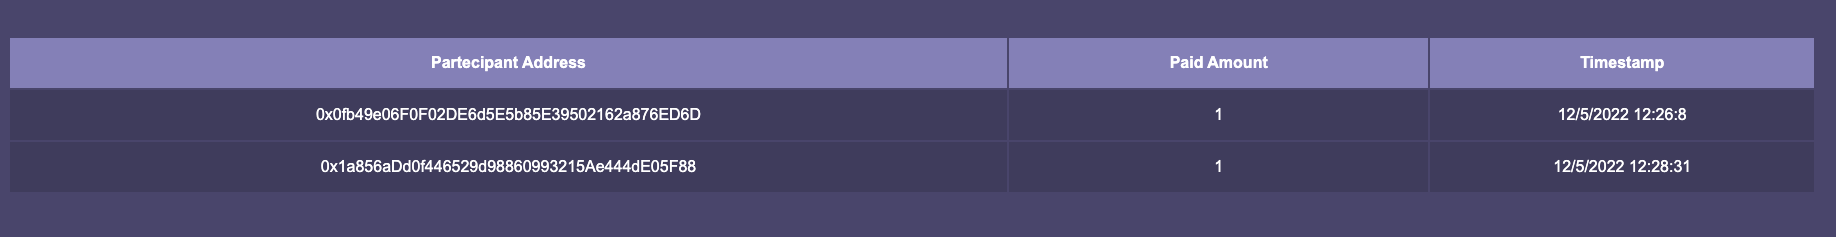
\includegraphics[scale=0.25]{immagini/Checkout/ContributionsTable.png} 
                \caption{Tabella dettaglio contribuenti}
            \end{figure}
            \begin{figure}[H]
                \centering
                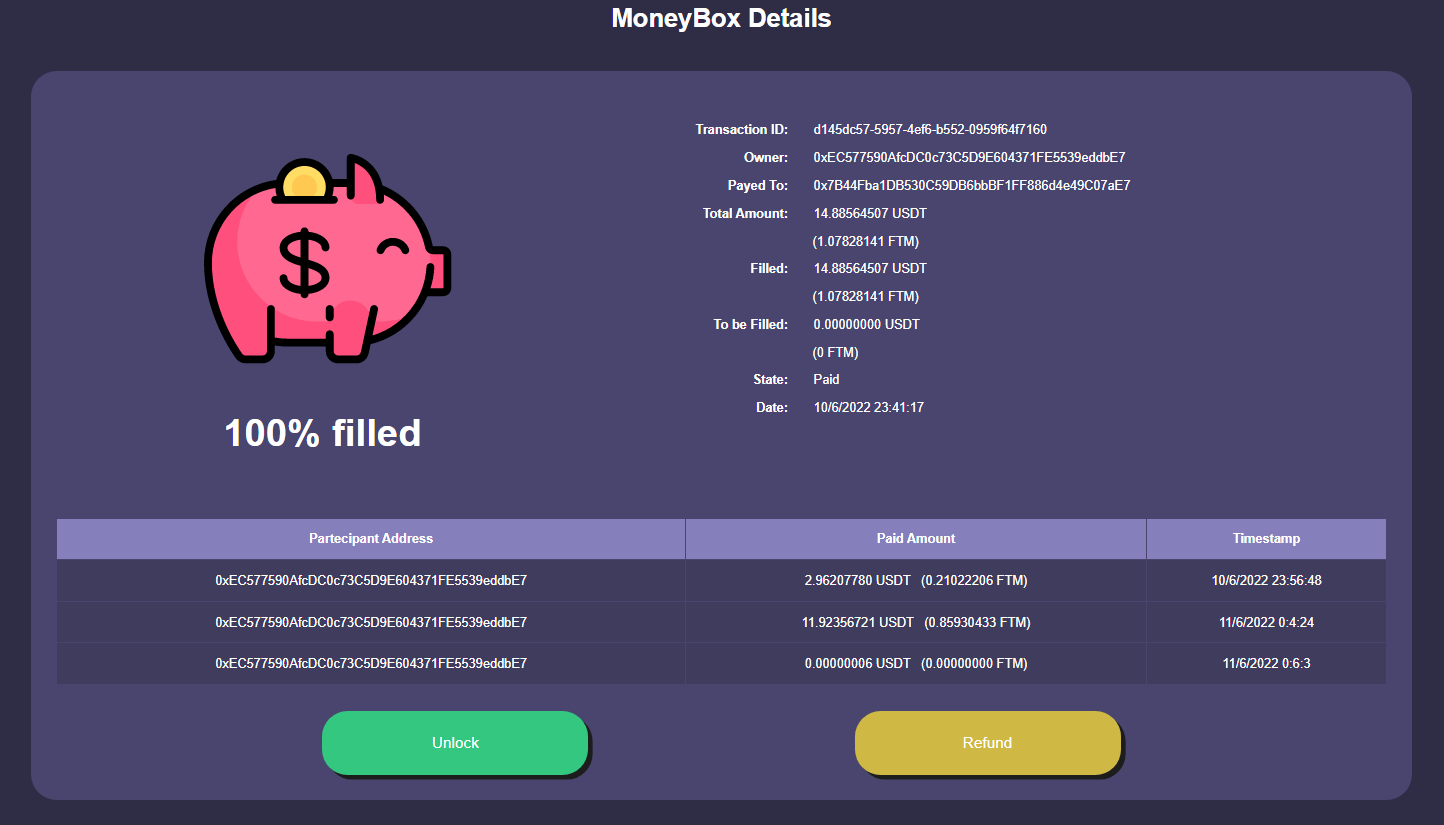
\includegraphics[scale=0.2]{immagini/Checkout/FilledMoneyBox.png} 
                \caption{Dettaglio MoneyBox in stato \texttt{"Paid"}}
            \end{figure}
            \textbf{}\\
            Da quest'ultima figura in particolare è possibile notare la comparsa del bottone di sblocco e la scomparsa del box per contribuire alla MoneyBox poiché, in quanto già piena, non è più possibile inserire denaro al suo interno.\\\\
            Da qui sarà quindi possibile sbloccare il denaro attraverso un codice di sblocco (una volta ricevuto l'ordine) o chiedere il rimborso (qualora l'ordine non venga mai recapitato) mediante gli appositi bottoni.
            \subsubsection{Sblocco e Rimborso}
       Sia nel caso di \texttt{sblocco} che nel caso di \texttt{rimborso}, al click dell'apposito bottone si aprirà un popup in quanto quella che si compie in questa fase è un'operazione irreversibile e dunque considerata sensibile.\\\\
        Nel caso di \textbf{sblocco} verrà mostrato un popup che mostrerà il codice di sblocco e un'input box nella quale replicare tale codice con l'aggiunta di due tasti per la conferrma dell'inserimento del codice o la chiusura del popup stesso:
        \begin{figure}[H]
            \centering
            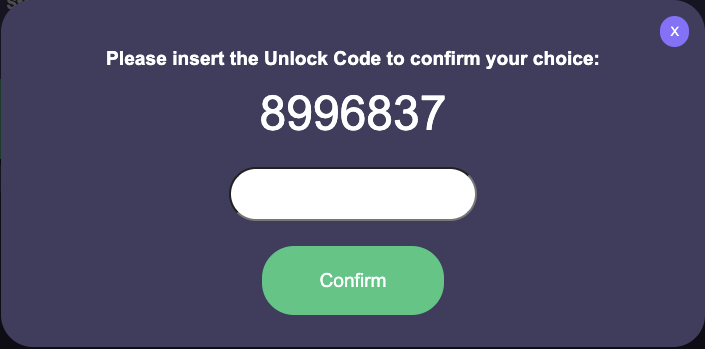
\includegraphics[scale=0.3]{immagini/Checkout/UnlockPopUp.png} 
            \caption{Popup di sblocco}
        \end{figure}
        \textbf{}\\
        Nel caso di \textbf{rimborso} verrà mostrato un semplice popup di conferma così da evitare pagamenti erronei.
        \begin{figure}[H]
            \centering
            \includegraphics[scale=0.3]{immagini/Checkout/RefundPopUp.png} 
            \caption{Popup di rimborso}
        \end{figure}

        \subsubsection{Transazioni}


            \paragraph{Dettagli della transazione}

            Dopo aver cliccato il bottone, all'utente verrà presentato il riepilogo dell'ordine, e verra messa a disposizione la possibilità
            di pagare interamente l'ordine o di creare una MoneyBox per lo stesso.

            %immagine pagina dettagli transazione

            \paragraph{Visualizzazione Transazioni}

            Tornando alla pagina Home, rimangono due bottoni nel menù di sinistra: "Your Transactions" e "Inbound Transactions".
            Cliccando su di essi si apriranno, rispettivamente, le pagine per visualizzare le transazioni in uscita dal proprio account e quelle in entrata.


                \subparagraph{Transazioni in uscita}

                \begin{figure}[H]
                    \centering
                    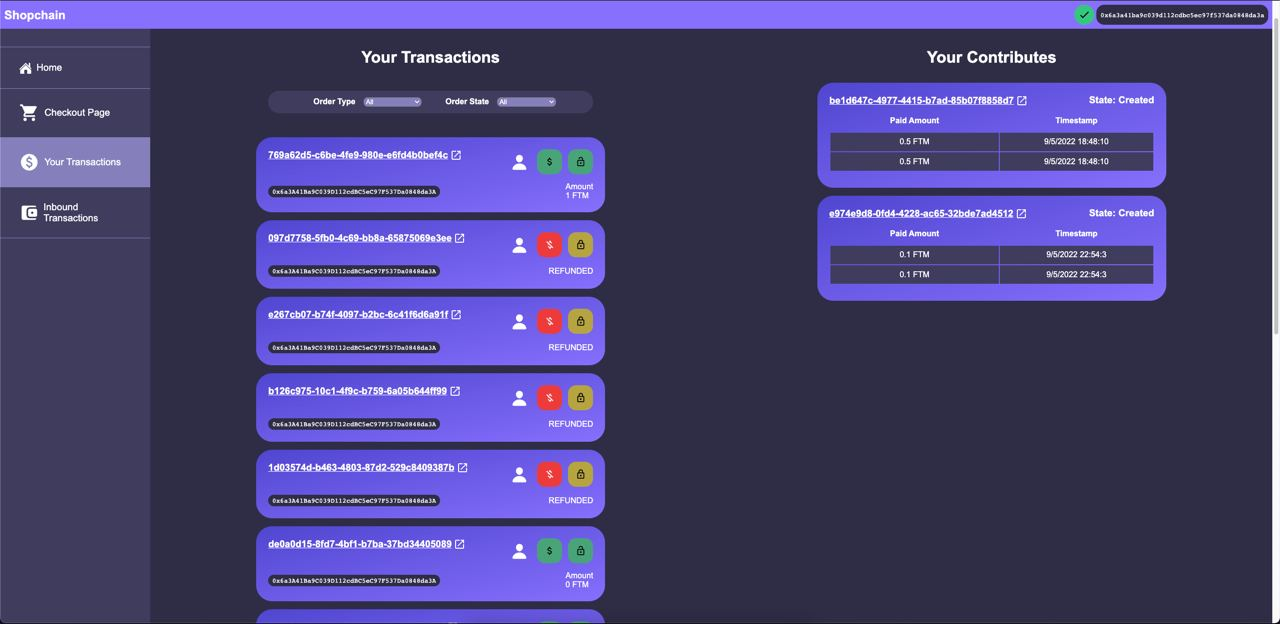
\includegraphics[scale=0.4]{immagini/Transaction/transactionview.jpg}
                    \caption{La vista delle transazioni in uscita}
                \end{figure}

                La pagina delle transazioni in uscita, "Your Transactions", è divisa in due sezioni:
                \begin{itemize}
                    \item Yuor Transactions: in questa sezione sono riportati gli ordini \textbf{creati} dall'utente;
                    \item Your Contributions: in questa sezione sono riportati gli ordini di tipo MoneyBox a cui l'utente ha pertecipato.
                \end{itemize}

                \paragraph{Transazioni in entrata}

                \begin{figure}[H]
                    \centering
                    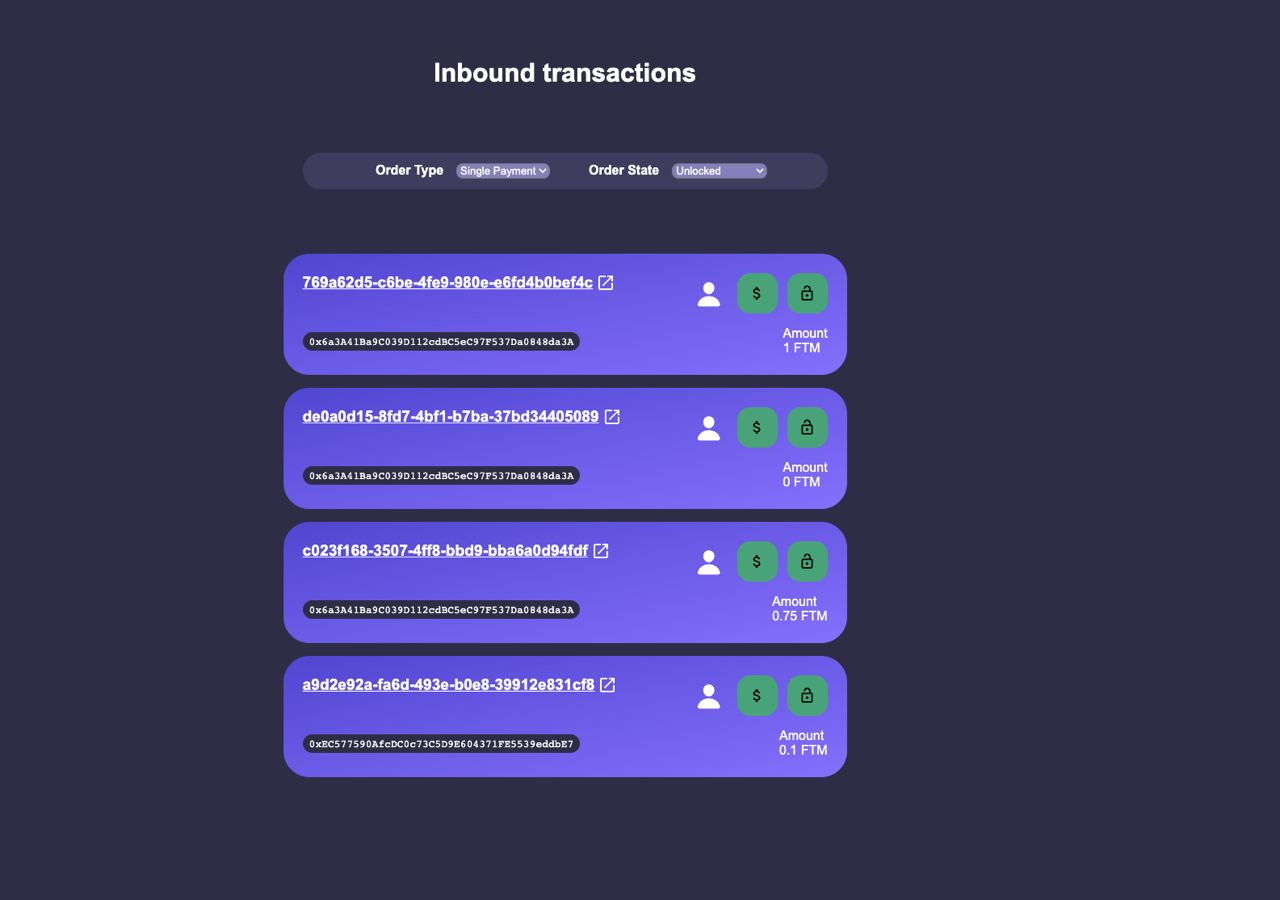
\includegraphics[scale=0.4]{immagini/Transaction/inboundtransactions.jpg}
                    \caption{La vista delle transazioni in entrata}
                \end{figure}

                Viceversa, la pagine delle transazioni in entrata, "Inbound Transactions", mostra solo una sezione con le transazioni effettuate verso il wallet dell'utente.

                \subparagraph{Ordinamento transazioni}

                L'applicazione offre la possibilità di ordinare l'elenco delle transazioni in due possibili modalità, combinabili tra loro: 
                "Order Type", il tipo dell'ordine, e "Order State", lo stato corrente dell'ordine.
                La scelta è effettuata tramite un apposito menu a tendina.

                \begin{figure}[H]
                    \centering
                    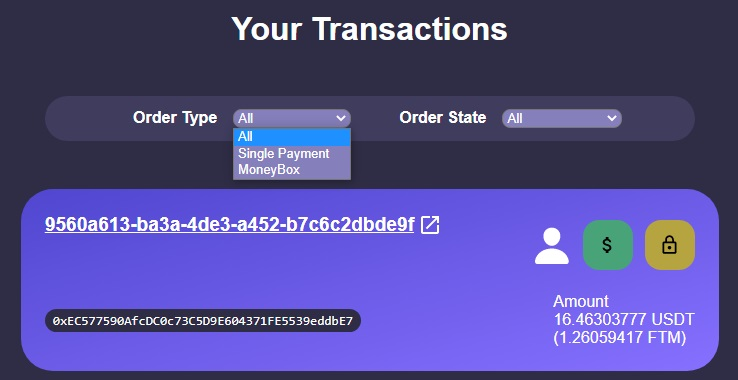
\includegraphics[scale=0.4]{immagini/Transaction/ordertype.jpg}
                \caption{Menu per la scelta del tipo di ordine}
                \end{figure}

                Il tipo di ordine potrà essere:
                \begin{itemize}
                    \item All: tutti i tipi di ordine;
                    \item Single Payment: pagamento singolo;
                    \item MoneyBox: pagamento creato come MoneyBox dall'utente.
                \end{itemize}

                \begin{figure}[H]
                    \centering
                    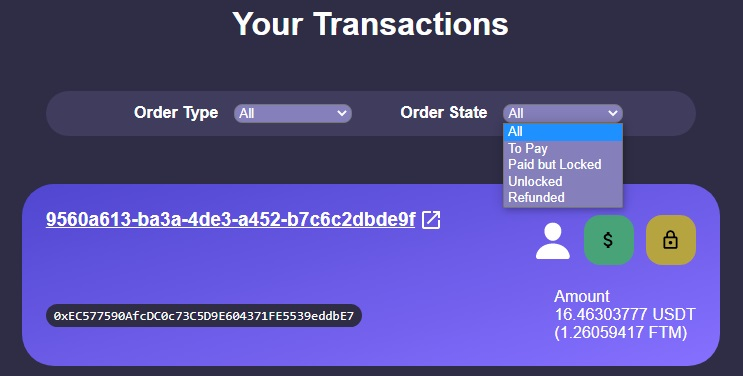
\includegraphics[scale=0.4]{immagini/Transaction/orderstate.jpg}
                    \caption{Menu per la scelta dello stato dell'ordine}
                \end{figure}

                Lo stato dell'ordine invece:
                \begin{itemize}
                \item All: tutti i tipi di stato;
                    \item To Pay: il pagamento deve ancora essere completato;
                    \item Paid but Locked: il pagamento è stato effettuato interamente, ma non ancora sbloccato;
                    \item Unlocked: il pagamento è stato effettuato e sbloccato;
                    \item Refunded: il pagamento è stato rimborsato.
                \end{itemize}

                L'ordinamento delle transazioni è disponibile sia per le transazioni in entrata che per quelle in uscita, e funziona in identico modo in entrambe le pagine.

                \paragraph{Transazione in dettaglio}

                \begin{figure}[H]
                    \centering
                    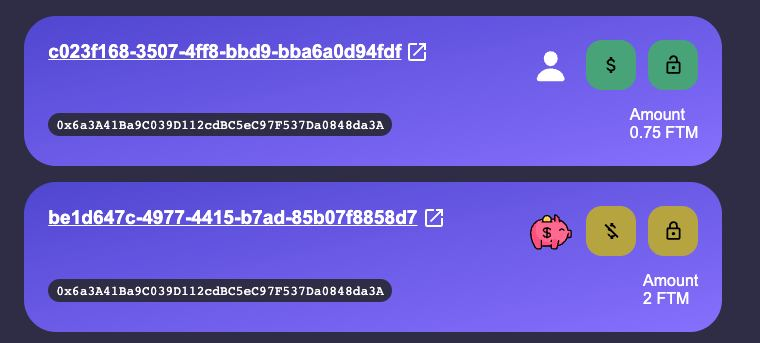
\includegraphics[scale=0.4]{immagini/Transaction/transactionsmall.jpg}
                    \caption{Due esempi di transazione nella lista "Your Transactions"}
                \end{figure}

                In dettaglio, le transazioni nelle liste sopracitate presentano all'utente le proprie informazioni più importanti.

                \begin{itemize}
                    \item l'id univoco del pagamento, cliccabile, che rimanda alla pagina di riepilogo dell'ordine, mostrata nella sezione ??;
                    \item l'indirizzo wallet dell'utente;
                    \item un'icona per identificare il tipo di pagamento, singolo o MoneyBox;
                    \item un'icona a forma di simbolo del dollaro per mostrare visivamente se la cifra richiesta è stata pagata interamente o meno;
                    \item un'icona a forma di lucchetto per mostrate visivamente lo stato del pagamento;
                    \item l'ammontare in FTM pagato.
                \end{itemize}

                L'icona di identificazione può assumere due forme: un icona di un uomo per il pagamento singolo, e l'icona di un maialino per il pagamento MoneyBox.

                \begin{figure}[H]
                    \centering
                    \begin{minipage}{0.45\textwidth}
                        \centering
                        
\includegraphics[scale=1]{immagini/uomo.jpg} 
                        \caption{Icona pagamento singolo}
                    \end{minipage}\hfill
                    \begin{minipage}{0.45\textwidth}
                    \centering
                        
\includegraphics[scale=1]{immagini/piggy.jpg} 
                        \caption{Icona pagamento MoneyBox}
                    \end{minipage}
                \end{figure}

                L'icona di stato dell'ammontare pagato può assumere i seguenti colori: \textbf{verde}, se l'ammontare richiesto è stato raggiunto, o \textbf{giallo} nel caso sia ancora da raggiungere.\\

                L'icona di stato del pagamento avrà un colore diverso a seconda dello stato corrente del pagamento: \textbf{verde} per i pagamenti effettuati e sbloccati, 
                \textbf{giallo} per i pagamenti completati non ancora sbloccati o non ancora interi, \textbf{rosso} per i pagamenti rimborsati.

